\chapter{Results}

Before discussing the results, you may want to describe the experimental setup: the dataset used, hardware platforms, hyperparameters, performance metrics, etc.

\section{Experiment 1}





\subsection{Weed Map Dataset}

\subsubsection{Introduction to Weed Map Dataset}

Weed Map Dataset is the dataset for the research “WeedMap: A large-scale semantic weed mapping framework using aerial multispectral imaging and deep neural network for precision farming” \cite{Tesi-2.1}.
\\[0.3cm]Each picture of the Dataset shows an image of a cultivated field, where there can been distinguished Dirt, Weeds and Crops.
\\[0.3cm]The image below (Fig.~\ref{fig:figure-2.1.1}) is an example on one of the images. It is first showed the entire Orthomosaic Map, and then different zoom levels. This puts in evidence the large scale of the image and the difficulty in distinguishing between Crops and Weeds.
\begin{figure}[t]
	\centering
	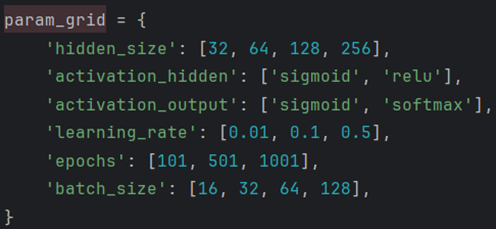
\includegraphics[width=14cm]{figures/figure-4.1.1.png}
	\caption[Example of image in Weed Map Dataset]{Example of image in Weed Map Dataset; with different zoom levels. Source:~\cite{Tesi-2.1}}
	\label{fig:figure-4.1.1}
\end{figure}

\myparagraph{Data Collection:}
The data included in the dataset was collected from aerial images (with Drones) from two different Sugar Beet fields: Eschikon (Switzerland) and Rheinbach (Germany). (Fig.~\ref{fig:figure-4.1.2})
\\[0.3cm]In particular, the utilized Drones are two commercial quadrotor UAV, equipped with multispectral cameras.
\begin{figure}[t]
	\centering
	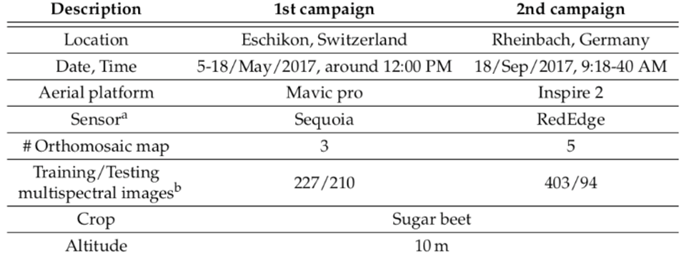
\includegraphics[width=13cm]{figures/figure-4.1.2.png}
	\caption[Information on Campaigns of Weed Map Dataset]{Information on the campaigns of data collection of Weed Map Dataset. Source:~\cite{Tesi-2.1}}
	\label{fig:figure-4.1.2}
\end{figure}

\subsubsection{Structure of Weed Map Dataset}

The full Dataset consist of 129 Directories for a total of 18746 images files. The total weight is 5.36GB.

\myparagraph{Folder Structure:}
There are two main folders, which are Orthomosaic and Tiles.
Orthomosaic contains the full orthomosaic maps.
Tiles contains, for each orthomosaic map, a folder containing images which represents cropped sections of the original orthomosaic map. All cropped sections together form the full map.
\\[0.3cm]Both Orthomosaic and Tiles contain RedEdge and Sequoia subfolders, containing 8 Orthomosaic maps in total (5 RedEdge and 3 Sequoia). (Fig.~\ref{fig:figure-4.1.3})
\\[0.3cm]Each Orthomosaic map stand in a folder indexed 000 to 007.
\begin{figure}[t]
	\centering
	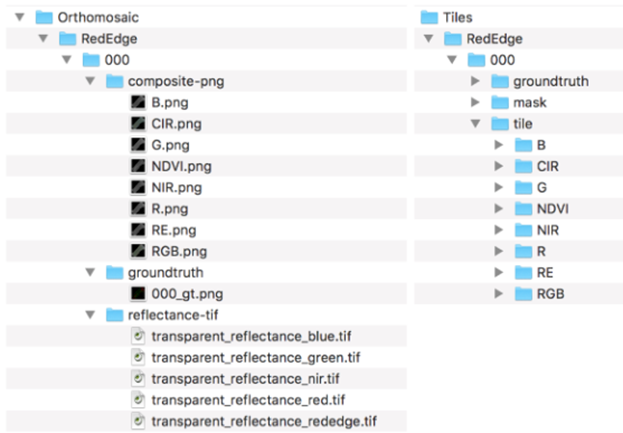
\includegraphics[width=10cm]{figures/figure-4.1.3.png}
	\caption[Folder Structure Weed Map Dataset]{Table showing the folder structure of Weed Map Dataset. Source:~\cite{Tesi-2.1}}
	\label{fig:figure-4.1.3}
\end{figure}

\myparagraph{Groundtruth:}
The Groundtruth images are pictures of the fields where each pixel has been manually labelled. (Fig.~\ref{fig:figure-4.1.4})
Each class is represented in a different colour:
\begin{itemize}[itemsep=0.1cm]
	\item Background (Dirt and part and part of the image which is not the crop field): is Black (code 0)
	\item Crops: is Green (code 1)
	\item Weeds: is Red (code 2)
\end{itemize}
The Groundtruth images are utilized to evaluate the precision of each prediction.
\begin{figure}[t]
	\centering
	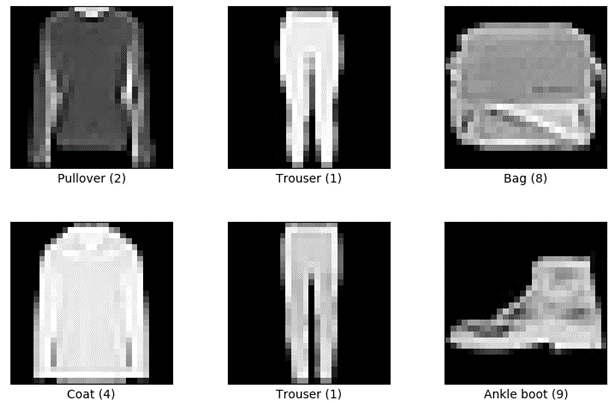
\includegraphics[width=5cm]{figures/figure-4.1.4.png}
	\caption[Example of GroundTruth in Weed Map Dataset]{Example of GroundTruth image in Weed Map Dataset. Source:~\cite{Tesi-2.1}}
	\label{fig:figure-4.1.4}
\end{figure}




\section{Experiment 2}

\lipsum  % Replace with your text
